% =========================================================================
\documentclass[aspectratio=1610]{beamer}

% ========================= Theme =========================================
\usetheme{Berkeley}
\usecolortheme{seahorse}

% ========================= Essential packages ============================
%\usepackage{hyperref}
%\hypersetup{
%    colorlinks = true,
%    linkcolor = blue,
%    citecolor = blue,
%    filecolor = blue,
%    urlcolor = blue
%}

% ========================= Frame notes systm ============================
\usepackage{xcolor}
\definecolor{codegreen}{rgb}{0,0.6,0}
\definecolor{codegray}{rgb}{0.5,0.5,0.5}
\definecolor{codepurple}{rgb}{0.58,0,0.82}
\definecolor{backcolour}{rgb}{0.95,0.95,0.92}
\usepackage{listings}
\lstdefinestyle{mystyle}{
    backgroundcolor=\color{backcolour},   
    commentstyle=\color{codegreen},
    keywordstyle=\color{black},
    numberstyle=\tiny\color{codegray},
    stringstyle=\color{black},
    basicstyle=\ttfamily\footnotesize,
    breakatwhitespace=false,         
    breaklines=true,                 
    captionpos=b,                    
    keepspaces=true,                 
    numbers=left,                    
    numbersep=5pt,                  
    showspaces=false,                
    showstringspaces=false,
    showtabs=false,                  
    tabsize=2
}

\lstset{style=mystyle}

% ========================= Plotting ======================================
\usepackage{calc}
\usepackage{tikz}
\usetikzlibrary{arrows,
                arrows.meta,
                calc,
		            chains,
                quotes,
                positioning,
		            shapes,
                shapes.geometric}
\usepackage{graphicx}
\usepackage{graphics}
\usepackage{pgfplots}
\pgfplotsset{width=7cm,compat=1.17}

%% ============================== Tabular =================================
\usepackage{booktabs}
\usepackage{tabularx,ragged2e}
\usepackage{array}
\usepackage{multirow}
\usepackage{siunitx}
  \sisetup{detect-all}
\usepackage{adjustbox}
\usepackage{rotating}
\usepackage{threeparttable}
\usepackage[justification=centering]{caption}

%% ============================== Text boxes ==============================
\usepackage[most]{tcolorbox}

%% ========================== Coding snippets =============================
% Default fixed font does not support bold face
%\usepackage{minted}
%\usemintedstyle{vs}

% ========================= Infor on authors ==============================
\title[Visual Forms]%
{Visual Forms}
\author{S.~Santoni\inst{1}}
\institute{
	\inst{1}%
	Bayes Business School
	}
\date{MSc in Business Analytics, 2024/25}

% ============================ Colors =====================================
\definecolor{base_c}{rgb}{0.6,0,0}
\definecolor{comp_c}{rgb}{0.09803921568627451, 0.6901960784313725, 0.7529411764705882}
\definecolor{tri_1}{rgb}{0.09803921568627451, 0.7686274509803922, 0.19215686274509805}
\definecolor{tri_2}{rgb}{0.19215686274509805, 0.09803921568627451, 0.7686274509803922}

% ========================= TOC  ==========================================
\AtBeginSection[]
{
	\begin{frame}
		       \frametitle{Outline}
		       \tableofcontents[currentsection,currentsubsection]
	\end{frame}
}

% ========================= References ===================================
\usepackage[style=numeric,backend=biber]{biblatex}
\addbibresource{bibliography.bib}

% =========================== TOC =========================================
\AtBeginSubsection[]
{
    \begin{frame}
        \frametitle{Outline}
        \tableofcontents[currentsection,currentsubsection]
    \end{frame}
}

% ========================= Document  ====================================
\begin{document}

\begin{frame}
	\titlepage
\end{frame}

\begin{frame}{Outline}
	\tableofcontents
\end{frame}

% ========================= Week 2 wrap up =================================
\section{Session \#2 Wrap Up}

\begin{frame}
	\frametitle{Grammar of Graphics}
	\begin{itemize}
		\item The Grammar of Graphics is an analytical framework that considers
		      the design of a chart as a `bundle of choices'
		\item Leland Wilkinson proposed GoF in 1999 \parencite{wilkinson2012grammar}
		\item Since then, many data visualization textbooks and packages have built
		      on it
		\item GoF advantages:
		      \begin{itemize}
			      \item GoF facilitates reasoning about a chart design
			      \item GoF is a discursive tool that help individuals discuss charts
		      \end{itemize}
	\end{itemize}
\end{frame}

\begin{frame}
	\frametitle{Software Adopting GoF}
	\framesubtitle{Python's Plotnine}
	\begin{figure}
		\begin{center}
			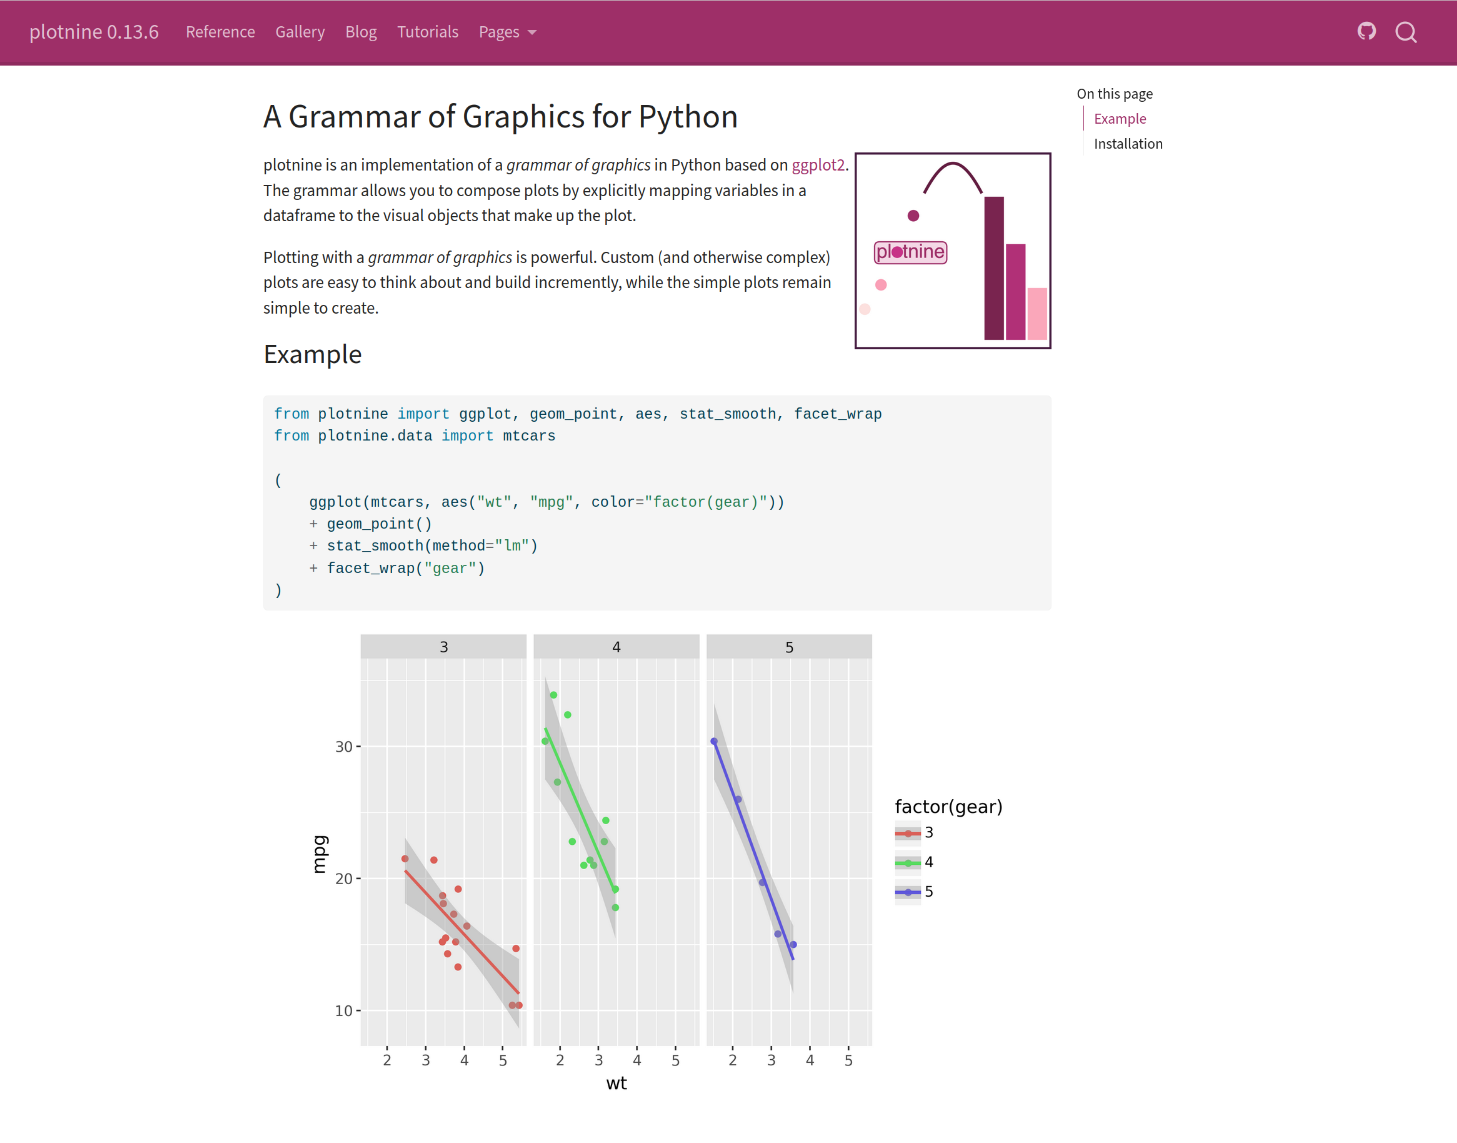
\includegraphics[width=0.7\textwidth]{figures/plotnine.png}
		\end{center}
	\end{figure}
\end{frame}

\begin{frame}
	\frametitle{Software Adopting GoF}
	\framesubtitle{Python's Vega-Altair}
	\begin{figure}
		\begin{center}
			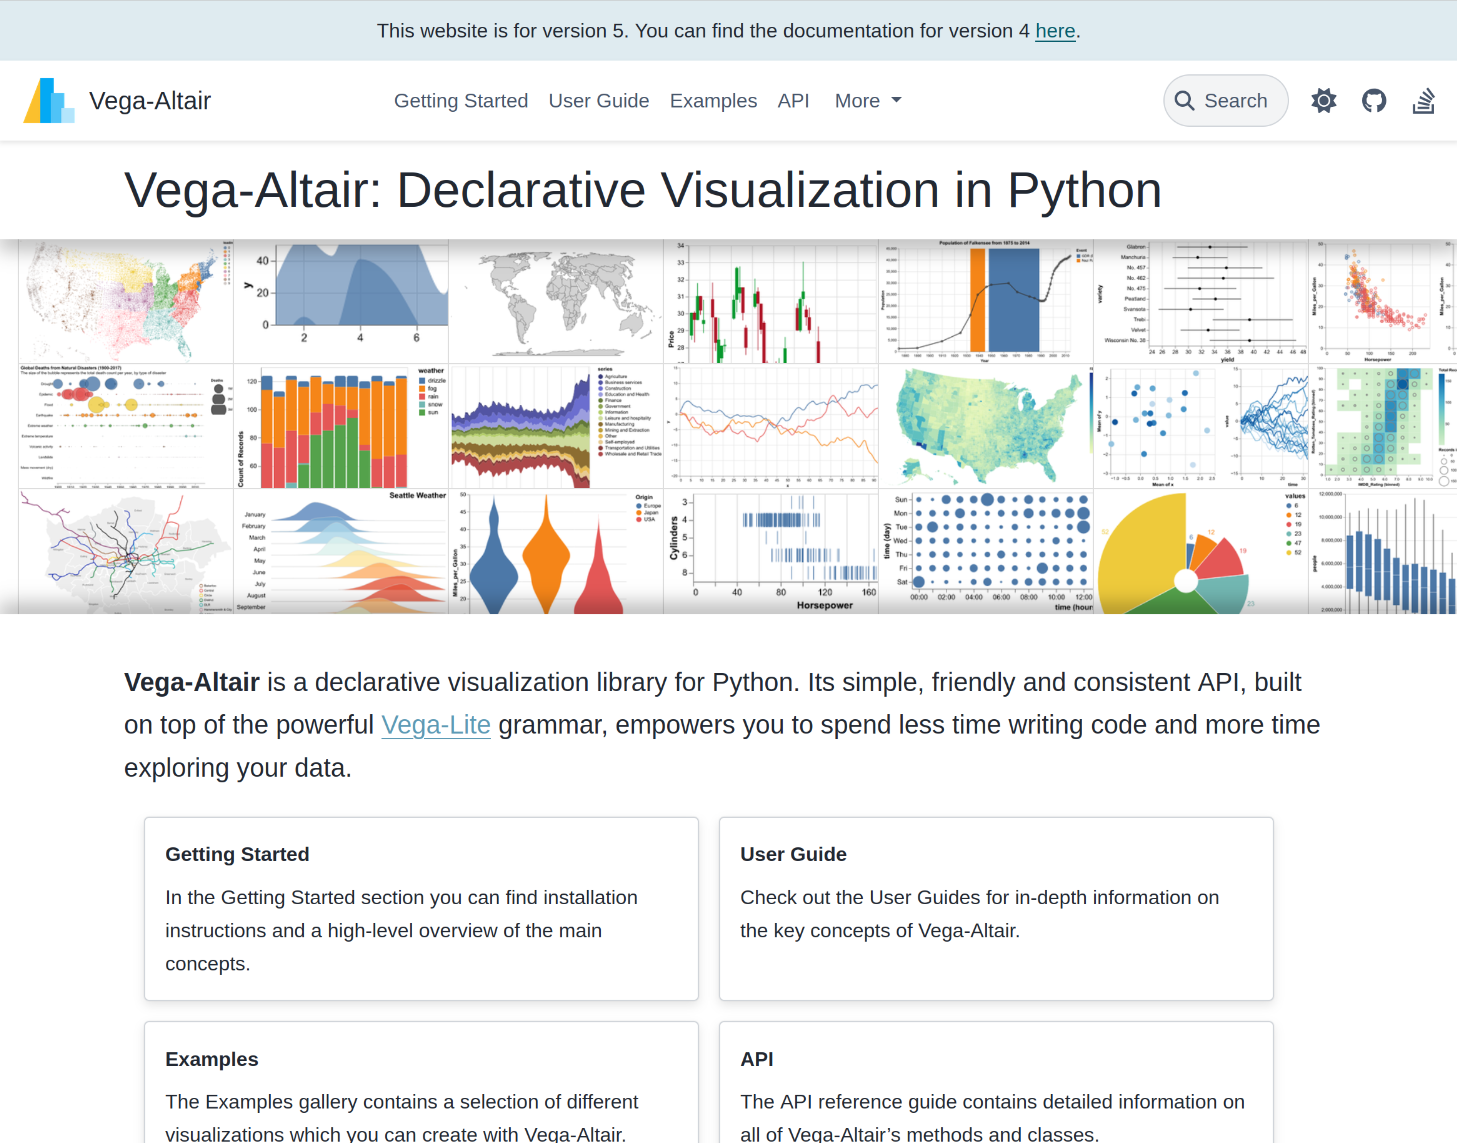
\includegraphics[width=0.7\textwidth]{figures/altair.png}
		\end{center}
	\end{figure}
\end{frame}

\begin{frame}
	\frametitle{Software Adopting GoF}
	\framesubtitle{Julia's Gadfly}
	\begin{figure}
		\begin{center}
			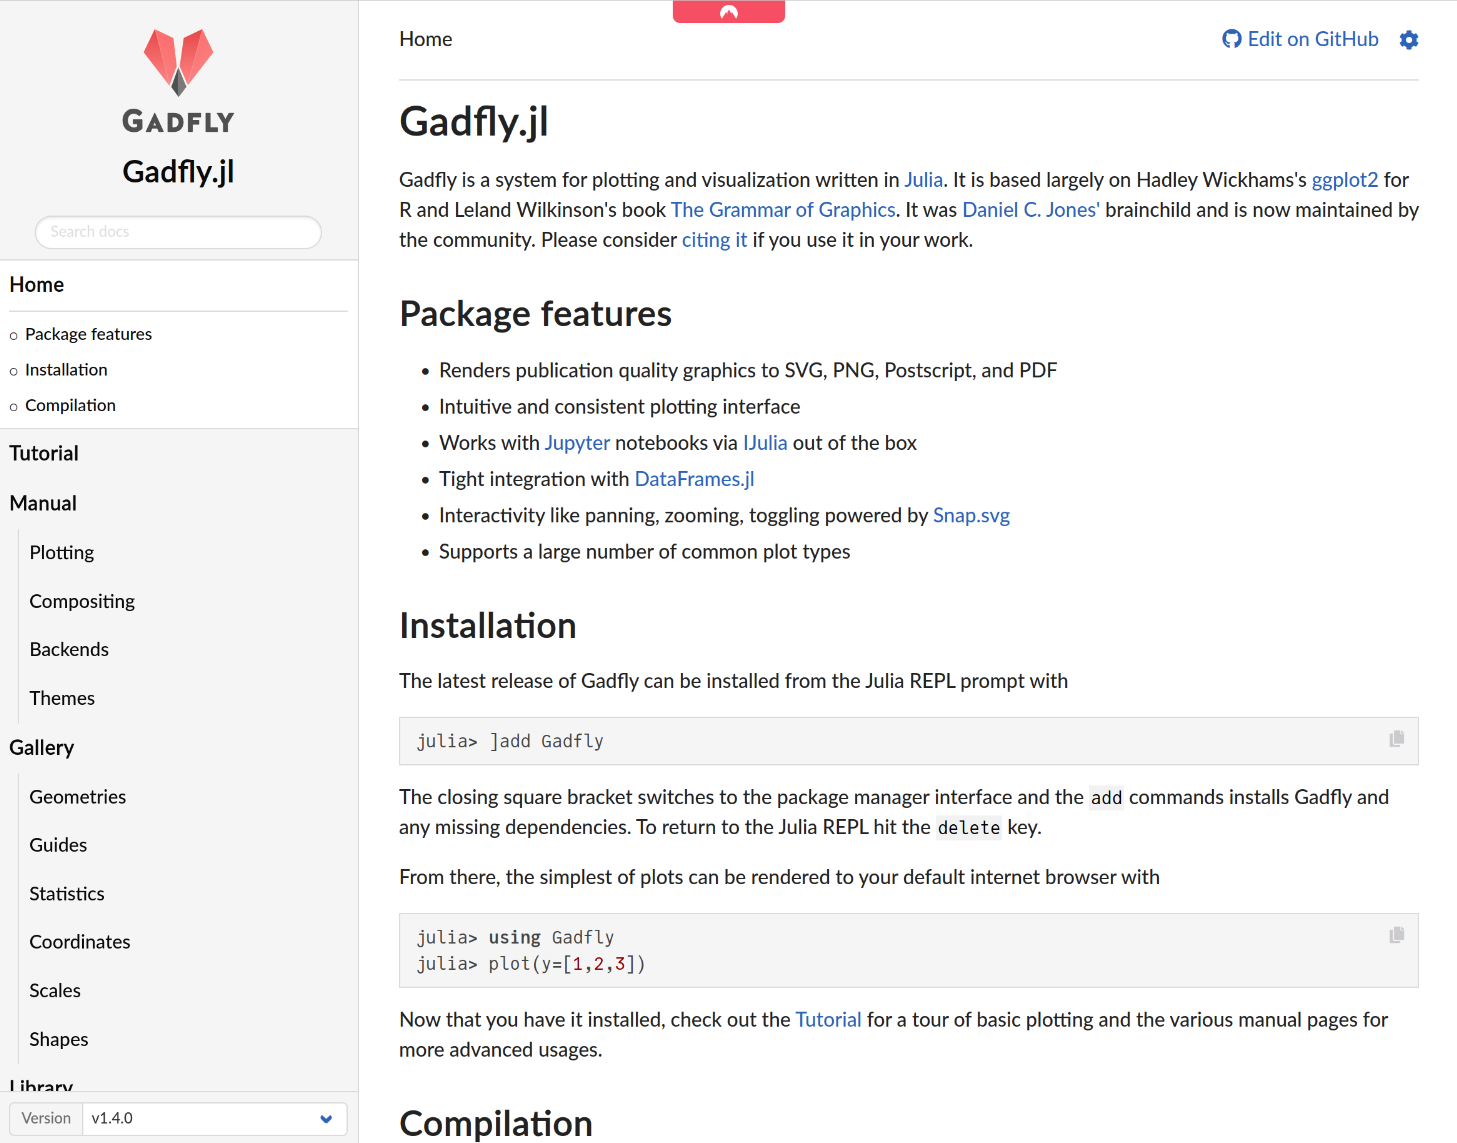
\includegraphics[width=0.7\textwidth]{figures/gadfly}
		\end{center}
	\end{figure}
\end{frame}

\begin{frame}
	\frametitle{Software Adopting GoF}
	\framesubtitle{R's \texttt{ggplot2}}
	\begin{figure}
		\begin{center}
			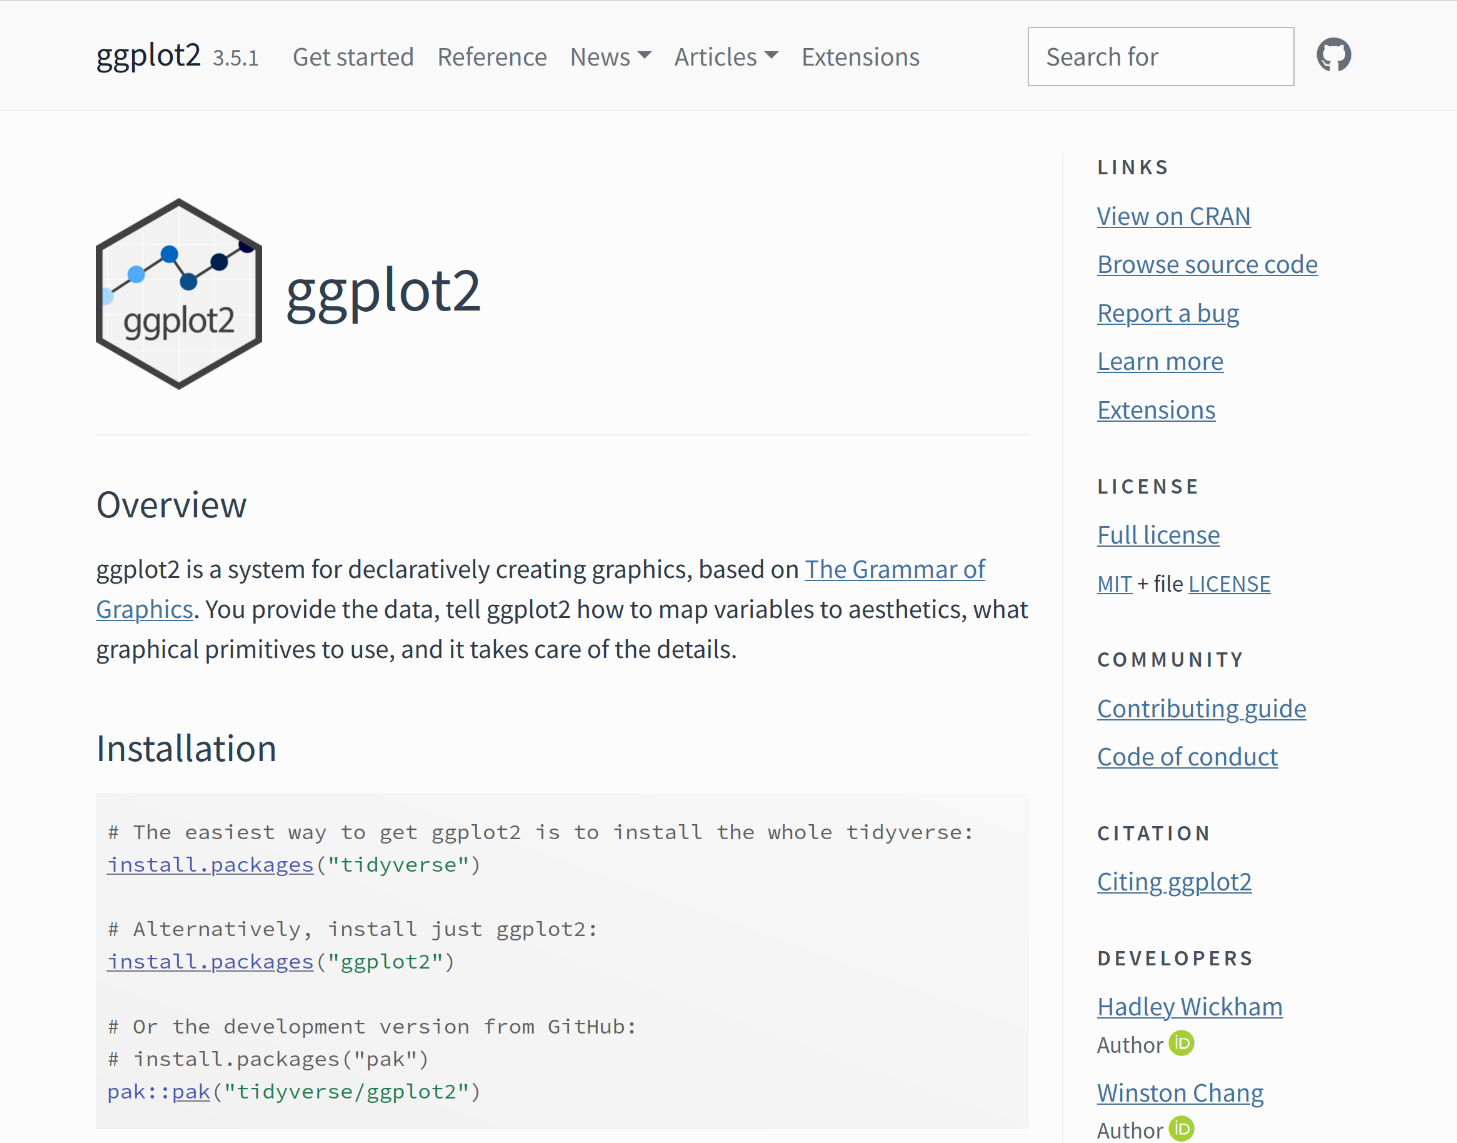
\includegraphics[width=0.7\textwidth]{figures/ggplot2.png}
		\end{center}
	\end{figure}
\end{frame}

\begin{frame}
	\frametitle{Porting GoF to Specific Software}
	\framesubtitle{Mapping between Wilkinson's GoF and \texttt{ggplot2}'s GoF}
	\begin{figure}
		\begin{center}
			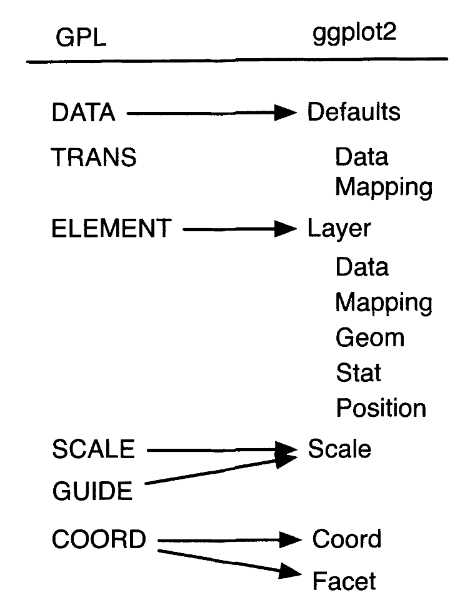
\includegraphics[width=0.35\textwidth]{figures/ggplot2_gof.png}
		\end{center}
	\end{figure}
	Source is \parencite{wickhamLayeredGrammarGraphics2010}
\end{frame}

\begin{frame}
	\frametitle{\texttt{ggplot2}'s Internal Structure}
	\begin{figure}
		\begin{center}
			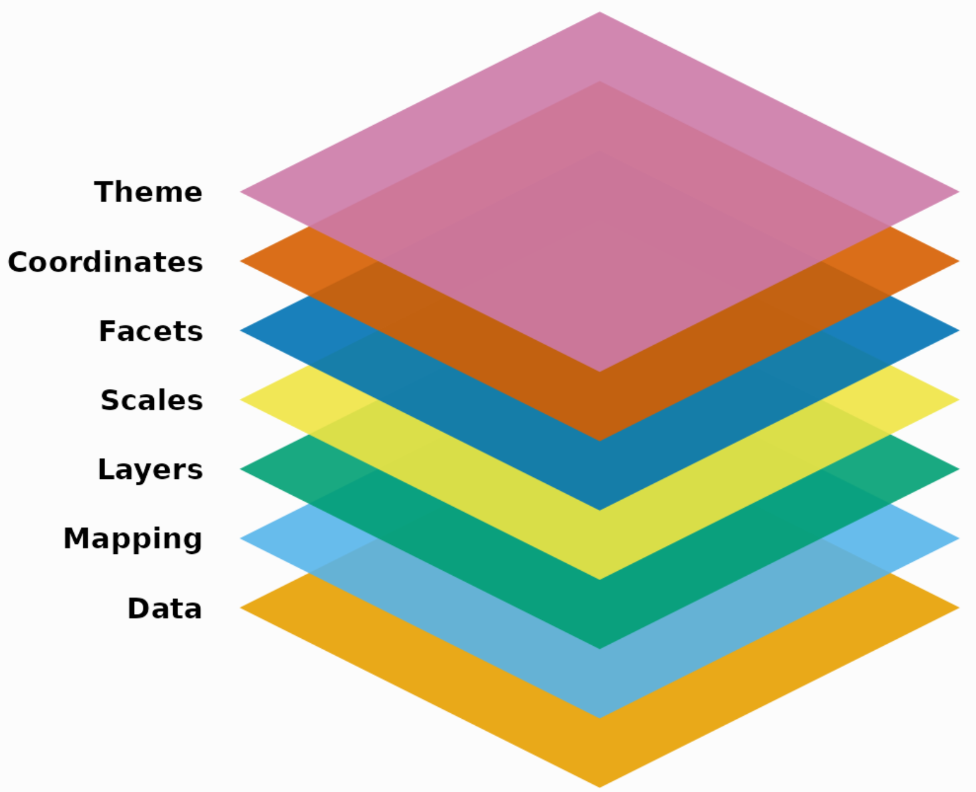
\includegraphics[width=0.6\textwidth]{figures/ggplot2_structure}
		\end{center}
	\end{figure}
	Source is \url{https://ggplot2.tidyverse.org/articles/ggplot2.html}
\end{frame}

\begin{frame}[fragile]
	\frametitle{A Minimal \texttt{ggplot2} Snippet}
	\begin{lstlisting}[language=R]
  library(ggplot2)

  ggplot(
    data = TIDYDATA,
    mapping = aes(x = COL_1, y = COL_2, colour = COL_3)
    ) +
    geom_point()
  \end{lstlisting}

\end{frame}

\begin{frame}[fragile]
	\frametitle{Data}
	\begin{quote}
		``The system works best if the data is provided in a tidy format, which
		briefly means a rectangular data frame structure where rows are observations
		and columns are variables.''

		\vspace{2em}

		``As the first step in many plots, you would pass the data to the ggplot()
		function, which stores the data to be used later by other parts of the
		plotting system.''

	\end{quote}

	\vspace{2em}

	\begin{lstlisting}[language=R]
  ggplot(data = TIDYDATA)
  \end{lstlisting}

\end{frame}

\begin{frame}[fragile]
	\frametitle{Mapping}

	\begin{quote}
		``The mapping of a plot is a set of instructions on how parts of the data are
		mapped onto aesthetic attributes of geometric objects. It is the ‘dictionary’
		to translate tidy data to the graphics system.''

	\end{quote}

	\vspace{2em}

	\begin{lstlisting}
  ggplot(data = TIDYDATA, mapping = aes(x = COL_1, y = COL_2))
  \end{lstlisting}

\end{frame}

\begin{frame}[fragile]
	\frametitle{Layers}

	\begin{quote}

		``The heart of any graphic is the layers. They take the mapped data and display it
		in something humans can understand as a representation of the data. Every layer
		consists of three important parts:

		\begin{enumerate}
			\item The geometry that determines how data are displayed, such as points, lines,
			      or rectanglesThe
			\item The statistical transformation that may compute new variables
			      from the data and affect what of the data is displayed
			\item The position adjustment that primarily determines where a piece of data
			      is being displayed.''
		\end{enumerate}
	\end{quote}
\end{frame}

% ========================== Visual forms =============================

\section{Visual Forms}

\begin{frame}
	\frametitle{What Are the Core Visual Forms in Data Visualization?}
	\begin{figure}
		\begin{center}
			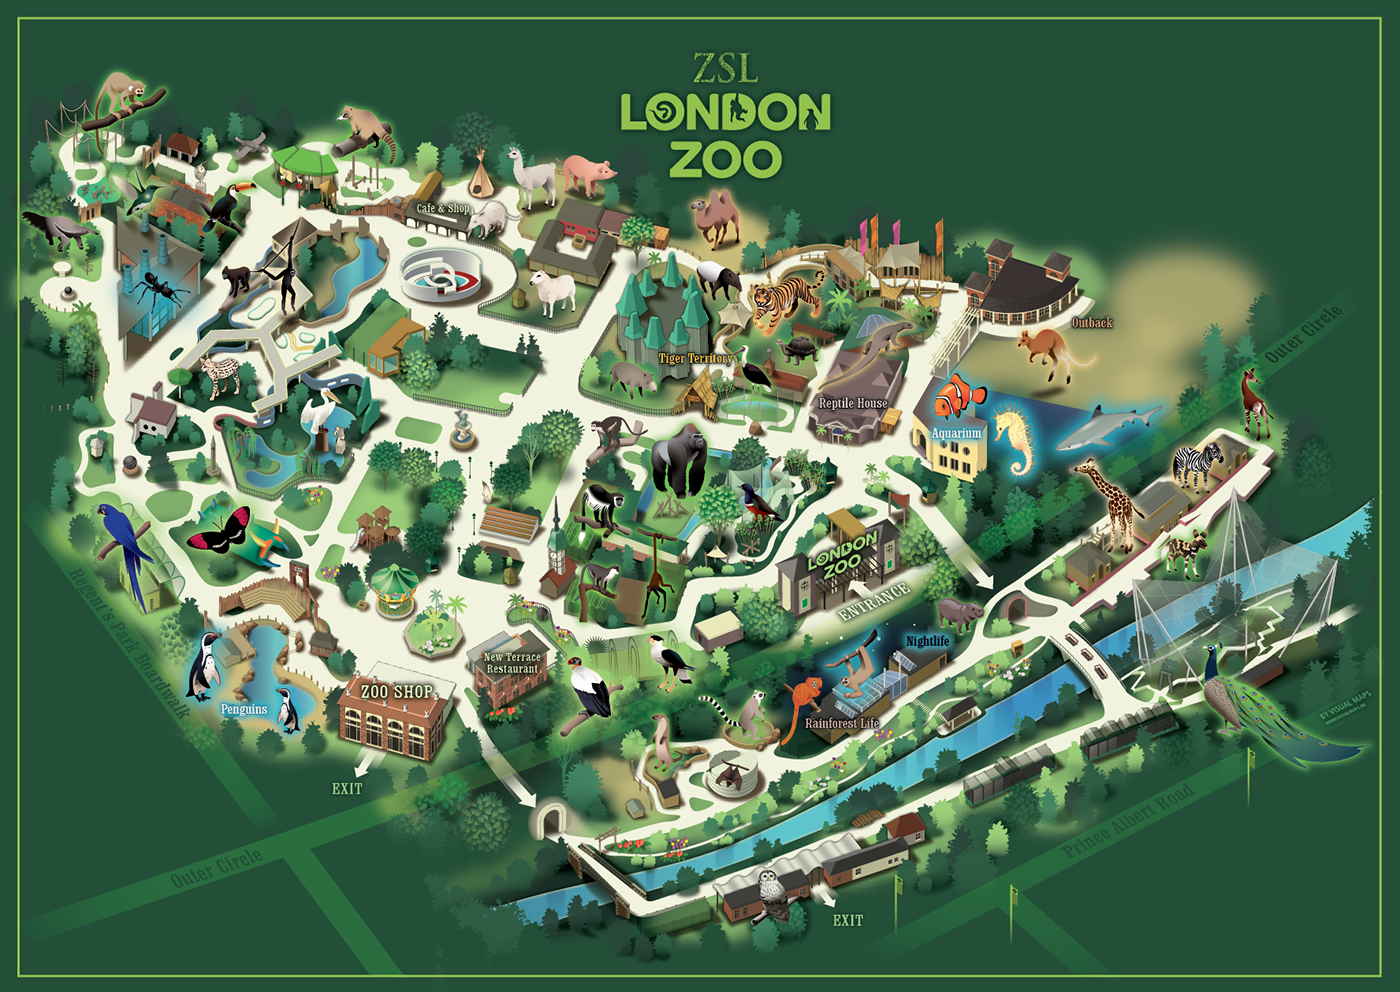
\includegraphics[width=0.8\textwidth]{figures/zoo.png}
		\end{center}
	\end{figure}
\end{frame}

\begin{frame}
	\frametitle{A Taxonomy of Visual Forms}
	\begin{columns}
		\column{0.45\textwidth}
		Cleveland \parencite{clevelandVisualizingData1993} proposes a taxonomy
		of the visual forms based on the cardinality of a plot's \textbf{mapping}
		$\Phi$:

		\begin{itemize}
			\item $||\Phi|| = 1 \rightarrow$ univariate plots
			\item $||\Phi|| = 2 \rightarrow$ bivariate plots
			\item $||\Phi|| = 3 \rightarrow$ trivariate plots
			\item $||\Phi|| \geq 4 \rightarrow$ hypervariate plots
		\end{itemize}
		\column{0.45\textwidth}
		\begin{figure}
			\begin{center}
				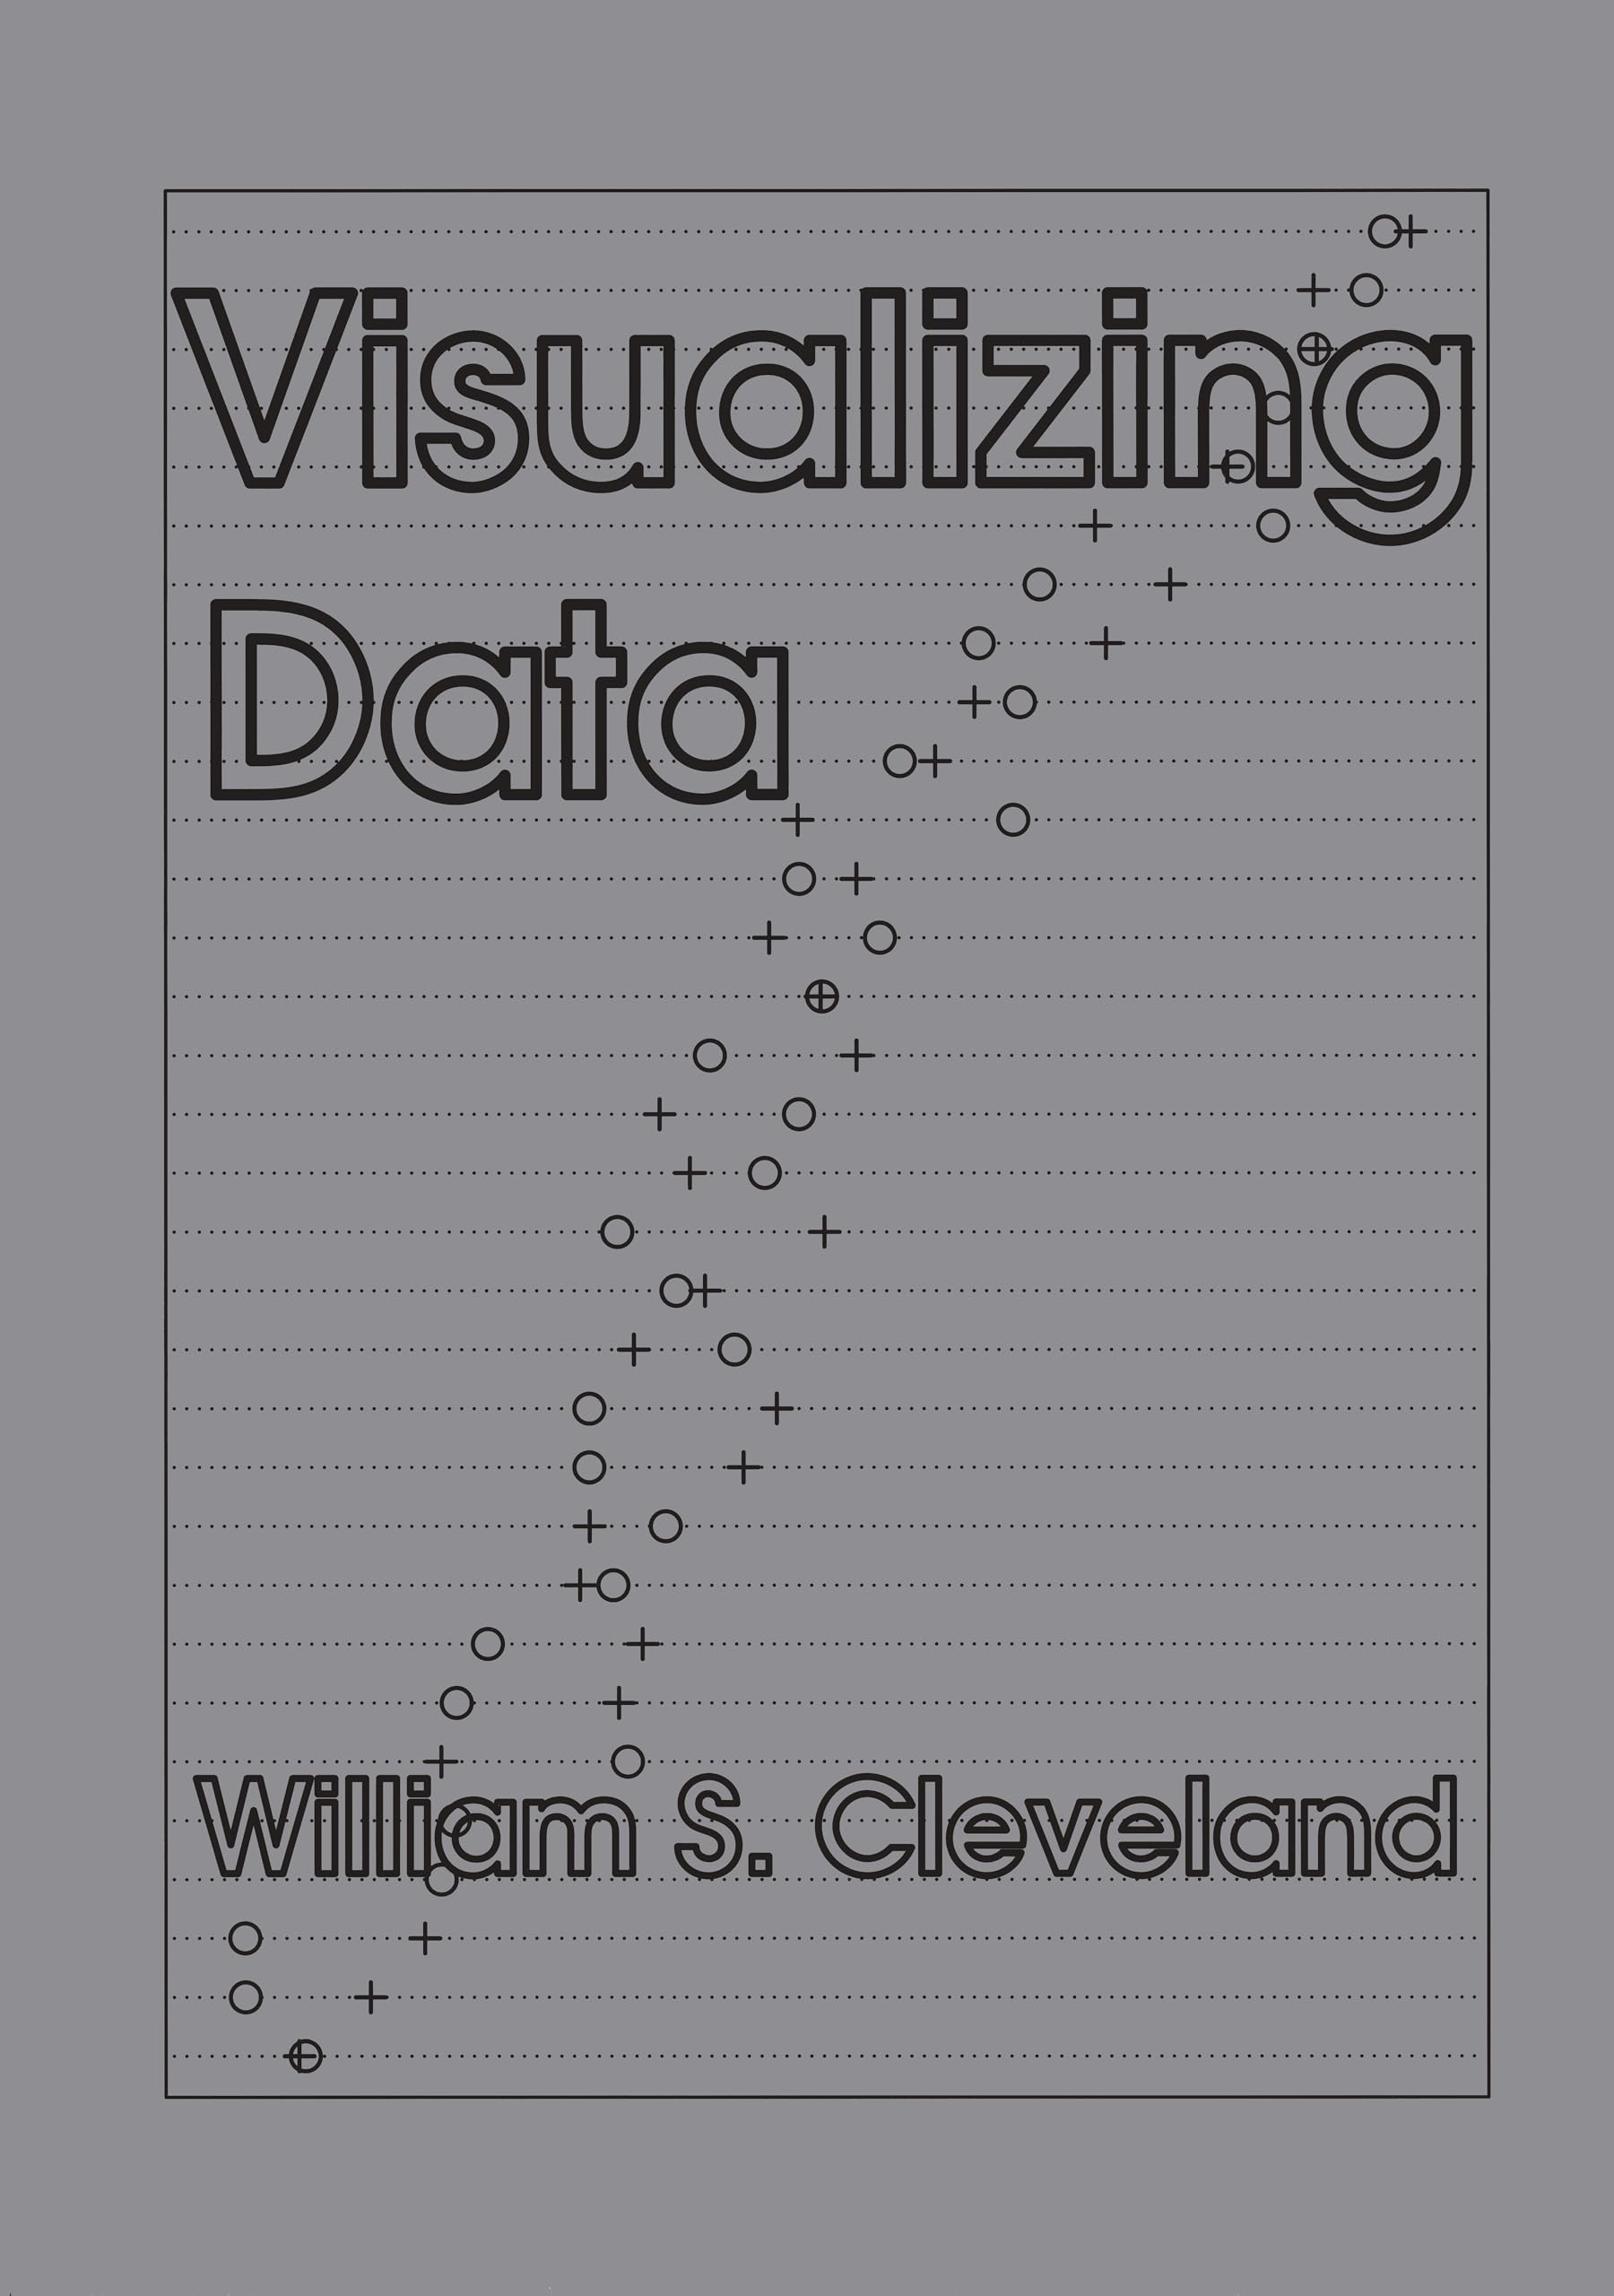
\includegraphics[width=0.8\textwidth]{figures/cleveland.jpg}
			\end{center}
		\end{figure}
	\end{columns}
\end{frame}


\subsection{Univariate plots}

\begin{frame}
\frametitle{}

\subsection{Bivariate plots}


\subsection{Trivariate plots}


\subsection{Hypervariate plots}



% ========================== Session 3 wrap up =============================
\section{Session \#3 Wrap Up}

\begin{frame}{}{}
	\LARGE \centering Time to wrap up!
\end{frame}

% =========================== Bibliography =================================
\begin{frame}
	\frametitle{References}
	\printbibliography
\end{frame}

\end{document}
